% Change the following title and label as desired.
\section{Literature Review}
\label{sec:literaturereview}

\subsection{Object Detection}
\label{subsec:detection}

\emph{Object detection} is a core technology in many modern applications such as surveillance systems, facial recognition, and autonomous vehicles. This technology is used to detect and classify various objects in images or videos. In the context of this research, \emph{object detection} plays a crucial role in detecting the presence of humans so that the autonomous wheelchair can follow the user's movements in real-time. Rapid advancements in \emph{deep learning}, especially with the use of \emph{Convolutional Neural Networks} (CNN), have optimized the capabilities of \emph{object detection}. \emph{CNN}, with its various layers such as convolutional, activation, pooling, and fully connected layers, forms the foundation of many current object detection methods, including \emph{YOLO} (You Only Look Once).

\subsection{Convolutional Neural Network (CNN)}
\label{subsec:cnn}

\emph{Convolutional Neural Network} (CNN) is a type of artificial neural network specifically designed for processing data with a grid-like structure, such as images. CNN consists of a series of layers that work together to extract and analyze features from input data, making it highly effective in tasks such as image classification, segmentation, and object detection \cite{oshea2015cnn}.

\begin{figure}[H]
  \centering
  \includegraphics[width=0.45\textwidth]{gambar/tex/simplecnn.pdf}
  \caption{An simple CNN architecture.}
  \label{fig:simplecnn}
  \end{figure}

\vspace{5pt}
\subsubsection{Convolutional Layer}
\label{subsubsec:Convolutional Layer}

The convolutional layer is the foundation of CNN that extracts important features from input images. By applying filters learned during training, this layer can recognize basic elements such as edges, textures, and patterns in images. Each filter in the convolutional layer is responsible for detecting specific features, and the results are organized into feature maps that provide a visual representation of the detected elements. The formula for the convolution operation can be written as follows:

\begin{equation}
  (f * g)(t) = \int_{-\infty}^{\infty} f(\tau)g(t - \tau) \, d\tau
\end{equation}

\vspace{5pt}
\subsubsection{Activation Layer}
\label{subsubsec:Activation Layer}

The activation layer is a component that adds non-linearity to the network, allowing the model to learn more complex relationships. Activation functions such as \emph{ReLU} (Rectified Linear Unit) are used to activate neurons only if their output is positive, thus reducing computational complexity and speeding up the training process. This non-linearity is crucial for addressing problems involving data with complex structures, such as object detection in images.

\vspace{5pt}
\subsubsection{Pooling Layer}
\label{subsubsec:Pooling Layer}

The pooling layer is used to reduce the dimensionality of feature maps while retaining the most relevant information. Pooling methods such as \emph{max pooling} take the maximum value within each pooling region, which helps the network become more robust to small variations in input, such as changes in scale or object rotation. By reducing the amount of data to be processed, pooling also helps to mitigate overfitting and speed up training. The max pooling operation can be represented as:

\begin{equation}
  P(x, y) = \max_{i,j \in \mathrm{PoolRegion}} I(x+i, y+j)
\end{equation}

\vspace{5pt}
\subsubsection{Fully Connected Layer}
\label{subsubsec:Fully Connected Layer}

The fully connected layer is the final layer in CNN that connects every neuron in the previous layer to every neuron in this layer. This layer serves to combine all the features extracted by the convolutional and pooling layers and produce the final output, such as object class predictions. The fully connected layer plays a crucial role in processing the information generated from the previous layers to make the final decision about classification or detection. The basic formula for the fully connected operation can be written as:

\begin{equation}
  y = f\left(\sum_{i=1}^{n} w_i x_i + b\right)
\end{equation}

Where \( w_i \) is the weight, \( x_i \) is the input, \( b \) is the bias, and \( f \) is the activation function.

\subsection{Pose Estimation}
\label{subsec:Pose Estimation}

\emph{Pose estimation} is a technique for identifying and tracking the position of the human body in images or videos. This technique typically involves detecting keypoints on the body, such as joints or limb extremities, which are used to model an individual's posture or movement. \emph{Pose estimation} is crucial in various applications, such as sports analysis, animation, and human-machine interaction. By utilizing \emph{pose estimation}, the system can understand the direction and intensity of the user's movements, allowing the wheelchair to respond appropriately and efficiently.

\subsection{YOLO (You Only Look Once)}
\label{subsec:YOLO}

\emph{YOLO}, developed by Joseph Redmon, introduces an \emph{End-to-End} approach for real-time object detection. The name \emph{YOLO}, which stands for \emph{"You Only Look Once"}, reflects the model's ability to complete the detection task with a single network pass. This is different from previous approaches that used sliding window techniques requiring classifiers to run multiple times on each image, or other methods that split the task into two separate steps: first, identifying regions that might contain objects (\emph{region proposals}), and second, running a classifier on the identified regions. Additionally, \emph{YOLO} uses a simpler output by employing regression to predict detection results, unlike methods such as \emph{Fast R-CNN} that separate the task into two outputs: classification probabilities and bounding box regression.

\vspace{5pt}
\subsubsection{YOLOv8}
\label{subsubsec:YOLOv8}

\emph{YOLOv8} is one of the highly efficient object detection models, combining high speed with relatively high accuracy. This architecture consists of several main layers: \emph{Backbone}, \emph{Neck}, and \emph{Head}. The \emph{Backbone} is responsible for extracting basic features from the input image. Then, the \emph{Neck} combines information from various layers to produce richer feature representations, which are then processed by the \emph{Head} to generate predictions for bounding boxes, class labels, and confidence scores.

\begin{figure}[H] 
  \centering 
  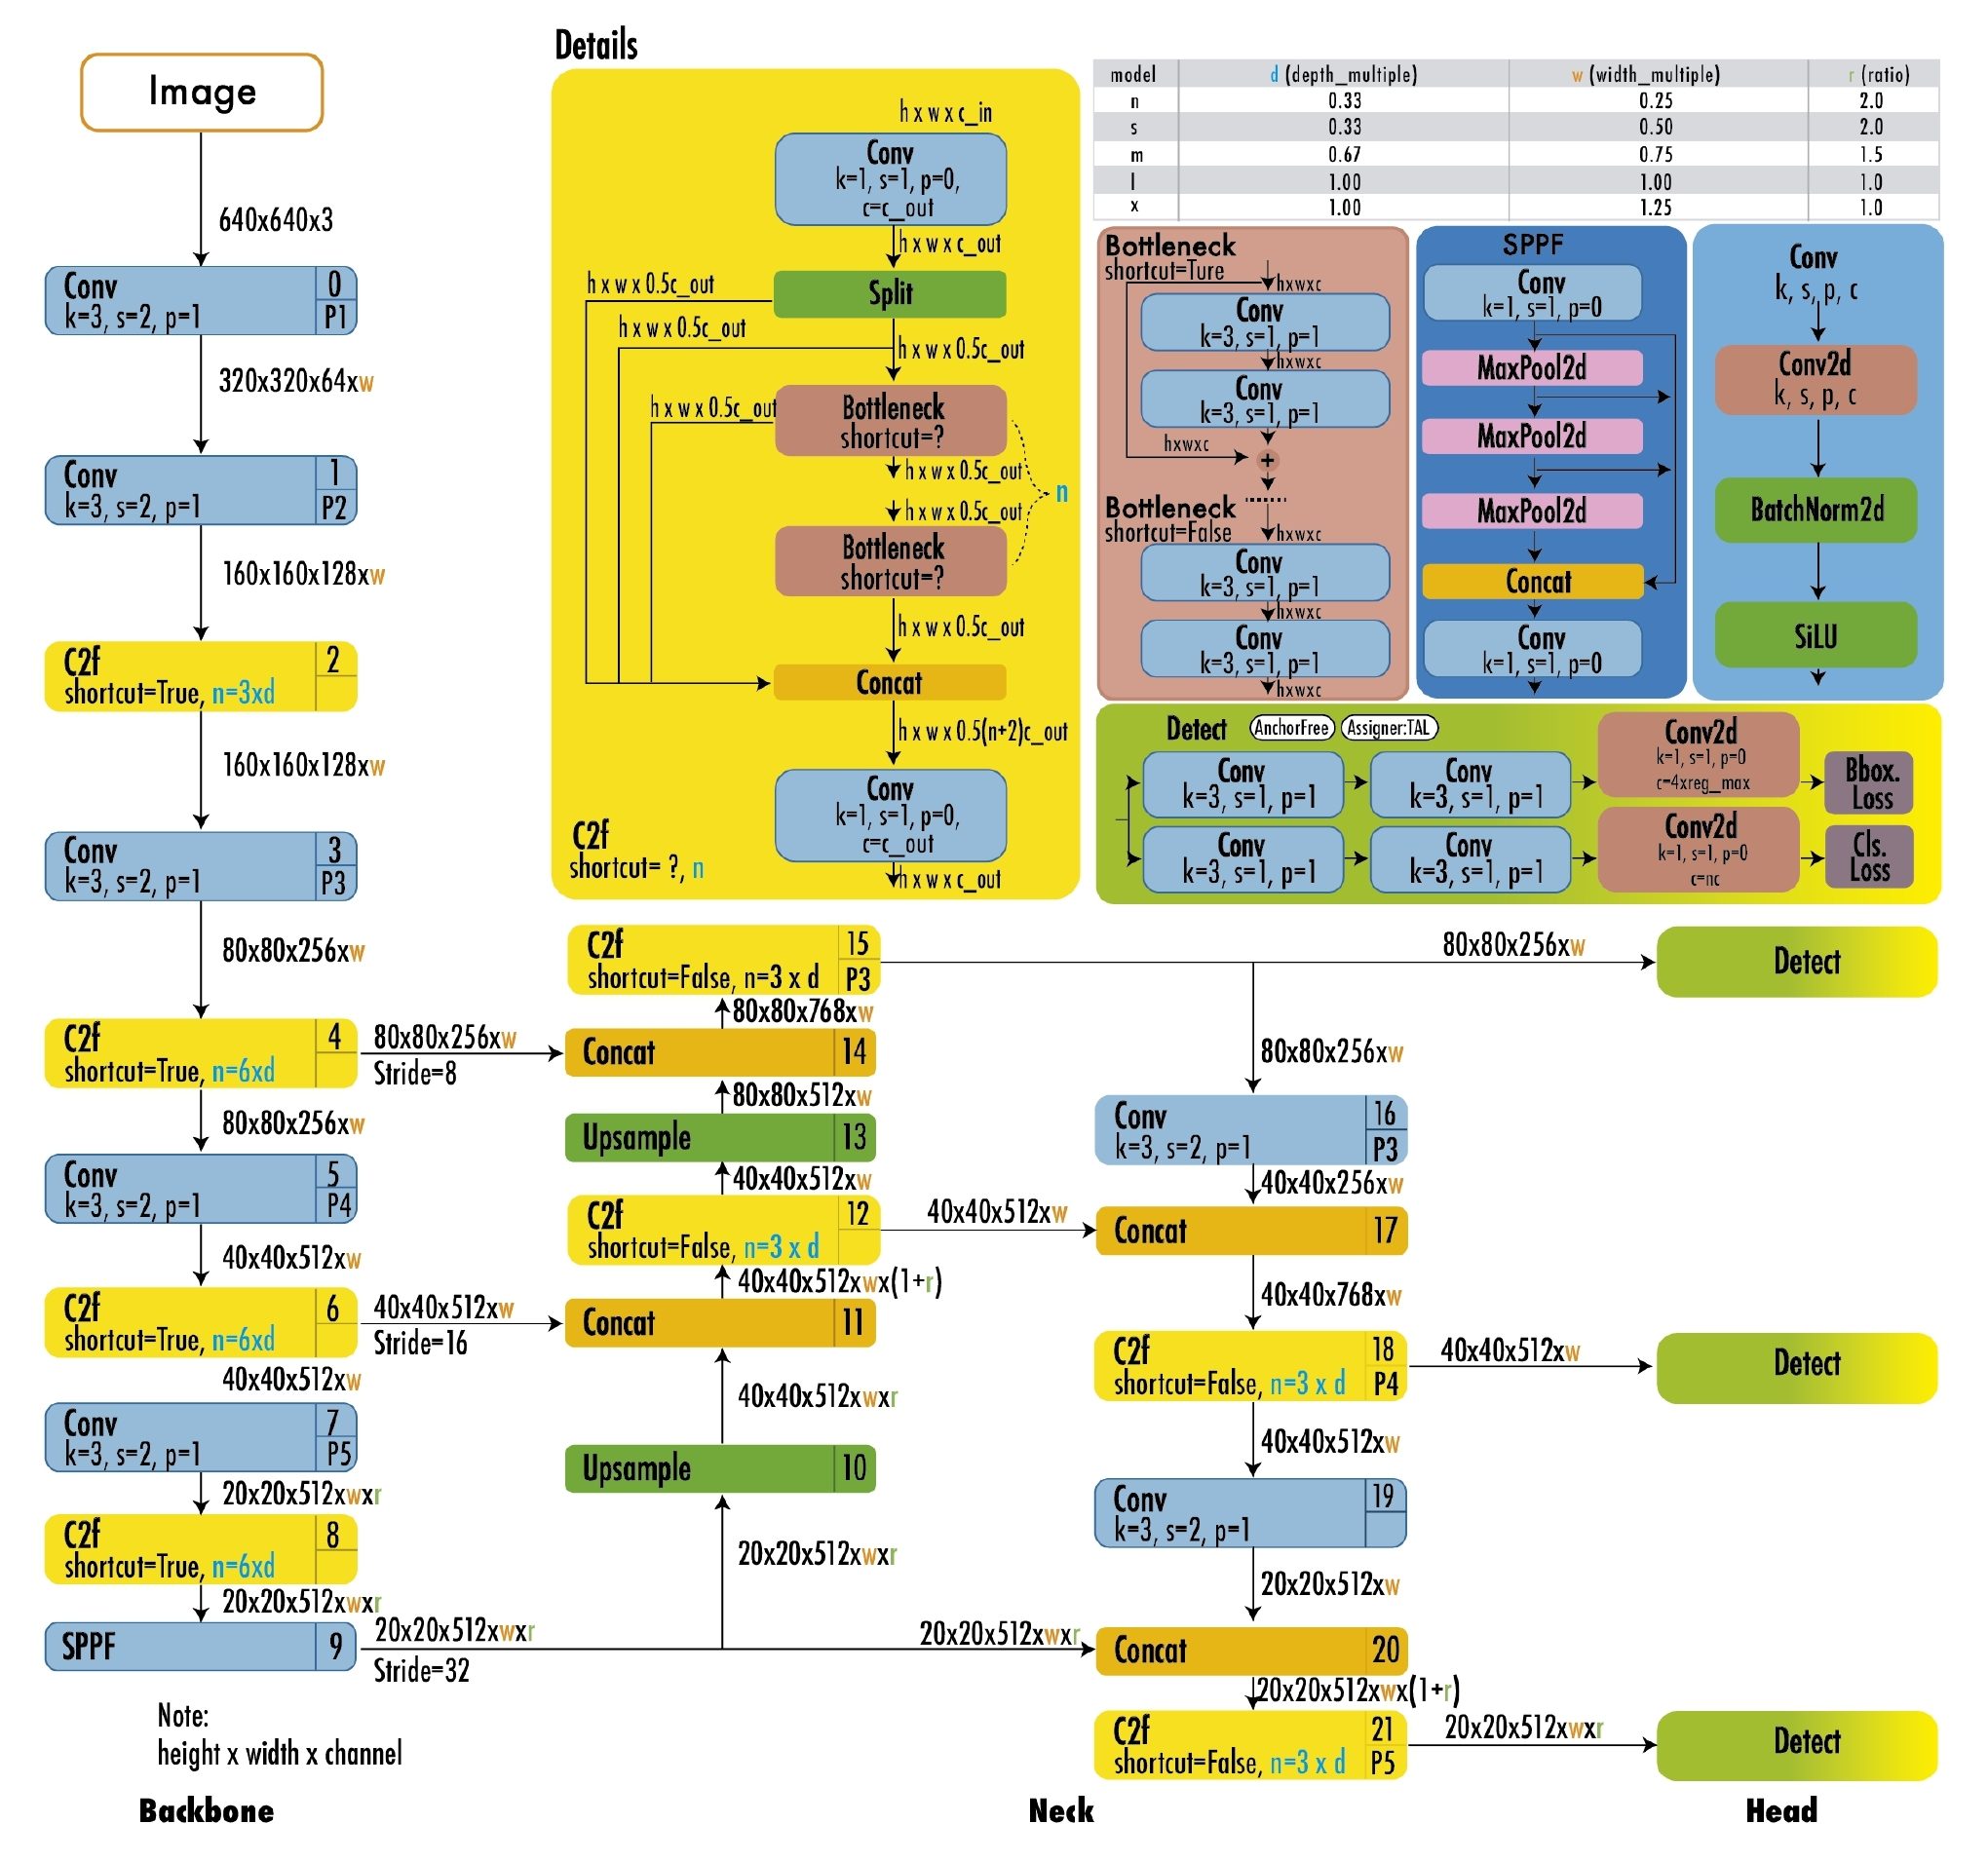
\includegraphics[scale=0.45]{gambar/YoloV8Architecture.jpg} 
  \caption{YOLOv8 Architecture.} 
  \label{fig:YOLOv8Architecture} 
\end{figure}

The figure shows the complete architecture of \emph{YOLOv8}, starting from the input image with a resolution of 640x640x3, which is processed through a series of convolutional layers in the \emph{Backbone} to extract important features. These features are then passed through the \emph{Neck}, which combines and processes information from various resolution levels, producing a rich multi-scale representation. Finally, the \emph{Head} is responsible for making the final predictions, such as bounding boxes, class labels, and confidence scores.

\emph{YOLOv8} predicts bounding boxes using a combination of center coordinates \((bx, by)\), bounding box dimensions \((bw, bh)\), and confidence score \(p_c\). The formula for calculating the bounding box coordinates based on the network output is:

\begin{equation}
  \begin{array}{c}
  bx = \sigma(t_x) + c_x\\
  bw = p_w e^{t_w}\\
  by = \sigma(t_y) + c_y\\ 
  bh = p_h e^{t_h}
  \end{array}
\end{equation}

Where \(t_x, t_y, t_w, t_h\) are the outputs of the neural network model, \(\sigma\) is the sigmoid function, \(c_x, c_y\) are the grid cell coordinates, and \(p_w, p_h\) are the anchor box scales.

The loss function in \emph{YOLOv8} consists of several main components that measure the difference between the model's predictions and the ground truth, balancing the importance of coordinate predictions, confidence scores, and object classification. The formula for the loss function is:

\begin{equation}
  \begin{array}{c}
  \mathbf{Loss} = \lambda_{\mathrm{coord}} \sum_{i=0}^{S^2} \sum_{j=0}^{B} \mathbb{1}_{ij}^{\mathrm{obj}} \left[ (bx_i - \hat{bx}_i)^2 + (by_i - \hat{by}_i)^2 \right] \\[10pt]
  + \lambda_{\mathrm{coord}} \sum_{i=0}^{S^2} \sum_{j=0}^{B} \mathbb{1}_{ij}^{\mathrm{obj}} \left[ (\sqrt{bw_i} - \sqrt{\hat{bw}_i})^2 + (\sqrt{bh_i} - \sqrt{\hat{bh}_i})^2 \right] \\[10pt]
  + \sum_{i=0}^{S^2} \sum_{j=0}^{B} \mathbb{1}_{ij}^{\mathrm{obj}} (C_i - \hat{C}_i)^2 + \lambda_{\mathrm{noobj}} \sum_{i=0}^{S^2} \sum_{j=0}^{B} \mathbb{1}_{ij}^{\mathrm{noobj}} (C_i - \hat{C}_i)^2 \\[10pt]
  + \sum_{i=0}^{S^2} \mathbb{1}_{i}^{\mathrm{obj}} \sum_{c \in \mathrm{classes}} (p_i(c) - \hat{p}_i(c))^2
  \end{array}
\end{equation}

In this equation, \(S\) is the grid size, \(B\) is the number of bounding boxes per grid cell, \(\mathbb{1}_{ij}^{\mathrm{obj}}\) is an indicator that bounding box j in cell i predicts an object, and \(\lambda_{\mathrm{coord}}\) and \(\lambda_{\mathrm{noobj}}\) are hyperparameters that control the importance of each loss component.

\vspace{5pt}
\subsubsection{YOLOv8 Pose}
\label{subsubsec: YOLOv8 Pose}

\emph{YOLOv8 Pose} is a variant of \emph{YOLOv8} specifically designed for pose estimation tasks. By combining the speed of \emph{YOLO} with precise pose detection capabilities, \emph{YOLOv8 Pose} can detect keypoints on the human body in real-time. Each bounding box not only contains information about the location and size of the object but also the coordinates of keypoints related to human pose (e.g., shoulders, elbows, knees, etc.).

\vspace{5pt}
\subsubsection{YOLOv10}
\label{subsubsec:YOLOv10}

\emph{YOLOv10} is a further development of \emph{YOLOv8}, with several improvements in efficiency and object detection accuracy. Like \emph{YOLOv8}, the \emph{YOLOv10} architecture consists of \emph{Backbone}, \emph{Neck}, and \emph{Head}, but with the addition of new modules such as \emph{Path Aggregation Network} (PSA) and \emph{Improved Convolutional Block} (C2fCIB).

The \emph{YOLOv10} architecture was developed by introducing several key enhancements from the foundations of \emph{YOLOv8}. The \emph{YOLOv10 Backbone} still functions as the main feature extractor but is enhanced with the \emph{SCD} (Squeeze-and-Excitation Convolutional Downsample) and \emph{C2fCIB} modules, which allow for more efficient information propagation and redundancy reduction. The newly added \emph{PSA} (Path Aggregation Network) module in the \emph{Neck} helps combine information from various paths within the network, enriching feature representation for multi-scale detection.

\vspace{5pt}
\subsubsection{YOLOv11}
\label{subsubsec:YOLOv11}

\emph{YOLOv11} is the latest breakthrough in the series of real-time object detectors from Ultralytics. Building on the advancements of its predecessors, \emph{YOLOv11} introduces significant improvements to its architecture, making it a powerful and adaptive solution for various computer vision applications. Ultralytics has introduced various enhancements in object detection and deep learning architecture. The improved \emph{backbone} and \emph{neck} architectures enhance feature extraction, enabling more accurate object detection and handling of more complex tasks.

Efficiency and speed are also sharpened through a refined architecture and a more optimal training pipeline, resulting in faster processing without sacrificing accuracy and performance. \emph{YOLOv11} supports implementation on various platforms, from edge devices, cloud platforms, to systems with NVIDIA GPUs, making it flexible for use in different environments. Additionally, \emph{YOLOv11} supports a variety of tasks, including object detection, instance segmentation, image classification, pose estimation, and oriented object detection (OBB). One of the main updates in the \emph{YOLOv11} architecture is the introduction of the \emph{C3K2} module, which replaces the \emph{C2F} module in \emph{YOLOv8}, as well as the addition of the \emph{C2PSA} module after the \emph{SPPF} module to further enhance detection capabilities.

\begin{figure}[H]
  \centering
  \resizebox{1\linewidth}{!}{
    \begin{tikzpicture}[node distance=1.5cm]
% Backbone Nodes
\node (input) [label] {Input};
\node (cbs0) [cbs, above of=input, yshift=1cm] {CBS\\k=3, s=2, p=1};
\node (cbs1) [cbs, above of=cbs0] {CBS\\k=3, s=2, p=1};
\node (c3k2_1) [c3k2, above of=cbs1] {C3K2\\C3k=Fa  lse};
\node (cbs2) [cbs, above of=c3k2_1] {CBS\\k=3, s=2, p=1};
\node (c3k2_2) [c3k2, above of=cbs2] {C3K2\\C3k=False};
\node (cbs3) [cbs, above of=c3k2_2] {CBS\\k=3, s=2, p=1};
\node (c3k2_3) [c3k2, above of=cbs3] {C3K2\\C3k=True};
\node (cbs4) [cbs, above of=c3k2_3] {CBS\\k=3, s=2, p=1};
\node (c3k2_4) [c3k2, above of=cbs4] {C3K2\\C3k=True};
\node (sppf) [layer, above of=c3k2_4, fill=green!20, align=center] {SPPF};
\node (c2psa) [layer, above of=sppf, fill=green!20, align=center] {C2PSA};

% Neck Nodes
\node (up1) [upsample, right of=sppf, xshift=2.25cm, minimum width=2cm] {Upsample};
\node (cc1) [concat, right of=up1, xshift=.5cm] {Concat};
\node (c3k2_5) [c3k2, right of=cc1, xshift=1cm] {C3K2\\C3k=False};

\node (up2) [upsample, below of=c3k2_5, minimum width=2cm] {Upsample};
\node (cc2) [concat, right of=up2, xshift=.5cm] {Concat};
\node (c3k2_6) [c3k2, right of=cc2, xshift=1cm] {C3K2\\C3k=False};

\node (cbs5) [cbs, above of=c3k2_6] {CBS\\k=3, s=2, p=1};
\node (cc3) [concat, right of=cbs5, xshift=1cm] {Concat};
\node (c3k2_7) [c3k2, right of=cc3, xshift=1cm] {C3K2\\C3k=False};

\node (cbs6) [cbs, above of=c3k2_7] {CBS\\k=3, s=2, p=1};
\node (cc4) [concat, right of=cbs6, xshift=1cm] {Concat};
\node (c3k2_8) [c3k2, right of=cc4, xshift=1cm] {C3K2\\C3k=True};

% Head Nodes
\node (detect1) [detect,  right of=c3k2_8, xshift=2cm] {Detect};
\node (detect2) [detect, below of=detect1] {Detect};
\node (detect3) [detect, below of=detect2] {Detect};

% SPPF Diagram
\node (cbs7) [cbs, right of=c3k2_3, xshift=4.75cm] {CBS \\ $k=1, s=1, p=1$};
\node (maxpool1) [layer, fill=red!30, below of=cbs7] {Maxpool};
\node (maxpool2) [layer, fill=red!30, below of=maxpool1] {Maxpool};
\node (maxpool3) [layer, fill=red!30, below of=maxpool2] {Maxpool};
\node (cc5) [concat, fill=blue!50, below of=maxpool3] {Concat};
\node (cbs8) [cbs, below of=cc5] {CBS \\ $k=1, s=1, p=1$};

% C2PSA Diagram
\node (cbs9) [cbs, right of=cbs7, xshift=4.75cm, yshift=.5cm] {CBS \\ $k=1, s=1, p=0$};
\node (split1) [layer, fill=cyan!30, below of=cbs9] {Split};
\node (PSA1) [layer, fill=purple!20, below of=split1] {PSABlock};
\node (dots) [label, below of=PSA1] {...};
\node (PSA2) [layer, fill=purple!20, below of=dots] {PSABlock};
\node (cc6) [concat, fill=blue!50, below of=PSA2] {Concat};
\node (cbs10) [cbs, below of=cc6] {CBS \\ $k=1, s=1, p=0$};

\node (attention) [layer, fill=cyan!30, right of=maxpool2, xshift=9.75cm] {Attention};
\node (cbs11) [cbs, below of=attention, yshift=-1.5cm] {CBS \\ $k=1, s=1, p=0$};
\node (cbs12) [cbs, below of=cbs11] {CBS \\ $k=1, s=1, p=0$};
\node (n1) [label, below of=cbs12] { };
\node (ffn) [label, above of=cbs11, xshift=-1cm, yshift=-.7cm] {FFN};
\node (h1) [label, above of=attention] { };

% CBS
\node (conv2d) [conv2D, right of=cbs9, minimum width=2cm, xshift=7.5cm] {Conv2D};
\node (bN) [layer, right of=conv2d, fill=orange!50, minimum width=1.5cm, xshift=.75cm] {BN};
\node (siLU) [layer, right of=bN, fill=yellow!50, minimum width=2cm, xshift=.75cm] {SiLU};

% Detection
\node (cbs22) [cbs, right of=PSA2, xshift=8cm] {CBS\\k=3, s=1, p=1};
\node (cbs21) [cbs, above of=cbs22] {CBS\\k=3, s=1, p=1};
\node (conv2d_1) [conv2D, below of=cbs22] {Conv2D};
\node (bbox) [layer, below of=conv2d_1, fill=red!50, minimum width=2cm,] {Bbox\\Loss};
\node (h2) [label, above of=cbs21] { };

\node (cbs31) [cbs, right of=cbs21, xshift=2cm] {CBS\\k=3, s=1, p=1};
\node (cbs32) [cbs, below of=cbs31] {CBS\\k=3, s=1, p=1};
\node (conv2d_2) [conv2D, below of=cbs32] {Conv2D};
\node (cls) [layer, below of=conv2d_2, fill=red!50, minimum width=2cm,] {Cls\\Loss};
\node (h3) [label, above of=cbs31] { };

% Labels
\node (Bone) [label, below of=cbs0, xshift=1.1cm] {Backbone};
\node (SPPF) [label, right of=Bone, xshift=5.1cm] {SPPF};
\node (C2PSA)[label, right of=SPPF, xshift=9.3cm] {C2PSA};
\node (PSABlock) [label, above of=C2PSA] {PSABlock};
\node (Detect) [label, right of=C2PSA, xshift=7.1cm] {Detect};
\node (CBS) [label, above of=Detect, yshift=8.3cm] {CBS};
\node (legend) [label, font=\small, left of=CBS, xshift=-2.8cm] {$kernel size(k), stride(s), padding(p)$};
\node (Head) [label, above of=CBS, yshift=1.2cm] {Head};
\node (Neck) [label, left of=Head, xshift=-1.7cm] {Neck};

% Blocks
\draw [dashed, thick, rounded corners] ($(cbs0.south west) - (.75,1.25)$) rectangle ($(c2psa.north east) + (.75,.75)$);
\draw [dashed, thick, rounded corners] ($(up1.south west) - (.25,2.25)$) rectangle ($(c3k2_8.north east) + (.25,.75)$);
\draw [dashed, thick, rounded corners] ($(detect3.south west) - (.75,.75)$) rectangle ($(detect1.north east) + (.75,.75)$);
\draw [dashed, thick, rounded corners] ($(conv2d.south west) - (.5,1)$) rectangle ($(siLU.north east) + (.75,.5)$);
\draw [dashed, thick, rounded corners] (2.5,.4) rectangle (8.5,12.75);
\draw [dashed, thick, rounded corners] (8.75,.4) rectangle (19.75,12.75);
\draw [dashed, thick, rounded corners] (15,1.9) rectangle (19.5,10);
\draw [dashed, thick, rounded corners] (20,.4) rectangle (27.75,10);

% Bracket for repeated layers
\draw [decorate, decoration={brace, amplitude=10pt}] 
    (14.2,9.5) -- (14.2,5) 
    node[midway, right=.3] {$n$};
\draw [decorate, decoration={brace, amplitude=10pt}] 
    ($(cbs21.north west)+(0,1)$) -- ($(cbs31.north east)+(0,1)$)
    node[midway, right=.3] { };

\draw [arrow] (maxpool1.west) -| +(-1.5,-1) |- (cc5);
\draw [arrow] (maxpool2.west) -| +(-1,-1) |- (cc5);
\draw [arrow] (maxpool3.west) -| +(-.5,-1) |- (cc5);
\draw [arrow] (split1.west) -| +(-1.5,-1) |- (cc6);
\draw [arrow] (PSA1.west) -| +(-1,-1) |- (cc6);
\draw [arrow] (PSA2.west) -| +(-.5,-1) |- (cc6);
\draw [arrow] (attention.south) |- +(0,-.5) -| ++(-2,0) |- ++(1,1.5) -| (attention.north);
\draw [arrow] (cbs12.south) |- +(0,-.5) -| ++(-2,0) |- ++(1,3.5) -| (cbs11.north);


% Arrows Backbone
\draw [arrow] (input) -- (cbs0);
\draw [arrow] (cbs0) -- (cbs1); 
\draw [arrow] (cbs1) -- (c3k2_1);
\draw [arrow] (c3k2_1) -- (cbs2);
\draw [arrow] (cbs2) -- (c3k2_2);
\draw [arrow] (c3k2_2) -- (cbs3);
\draw [arrow] (cbs3) -- (c3k2_3);
\draw [arrow] (c3k2_3) -- (cbs4);
\draw [arrow] (cbs4) -- (c3k2_4);
\draw [arrow] (c3k2_4) -- (sppf);
\draw [arrow] (sppf) -- (c2psa);

% Arrows Neck
\draw [arrow] (c3k2_3.east) -| +(.25,0) |- +(1,3.75) -| (cc1);
\draw [arrow] (c3k2_2.east) -| +(.5,0) |- +(1,5.25) -| (cc2);
\draw [arrow] (c3k2_5.north) |- +(1,.25) -| (cc3);
\draw [arrow] (c2psa.north) |- +(1,.25) -| (cc4);
\draw [arrow] (c2psa.north) |- +(1,.25) -| (up1);
\draw [arrow] (c3k2_5) -- (up2);
\draw [arrow] (c3k2_6) -- (cbs5);
\draw [arrow] (c3k2_7) -- (cbs6);

% Arrow Head
\draw [arrow] (c3k2_8) -- (detect1);
\draw [arrow] (c3k2_7) -- (detect2);
\draw [arrow] (c3k2_6) -- (detect3);

\draw [arrow] (cbs7) -- (maxpool1);
\draw [arrow] (maxpool1) -- (maxpool2);
\draw [arrow] (maxpool2) -- (maxpool3);
\draw [arrow] (maxpool3) -- (cc5);
\draw [arrow] (cc5) -- (cbs8);

\draw [arrow] (cbs9) -- (split1);
\draw [arrow] (split1) -- (PSA1);
\draw [arrow] (PSA1) -- (dots);
\draw [arrow] (dots) -- (PSA2);
\draw[arrow] (PSA2) -- (cc6);
\draw[arrow] (cc6) -- (cbs10);

\draw[arrow] (h1) -- (attention);
\draw[arrow] (attention) -- (cbs11);
\draw[arrow] (cbs11) -- (cbs12);
\draw[arrow] (cbs12) -- (n1);

\draw[arrow] (conv2d) -- (bN);
\draw[arrow] (bN) -- (siLU);

\draw[arrow] (h2) -- (cbs21);
\draw[arrow] (cbs21) -- (cbs22);
\draw[arrow] (cbs22) -- (conv2d_1);
\draw[arrow] (conv2d_1) -- (bbox);

\draw[arrow] (h3) -- (cbs31);
\draw[arrow] (cbs31) -- (cbs32);
\draw[arrow] (cbs32) -- (conv2d_2);
\draw[arrow] (conv2d_2) -- (cls);
\end{tikzpicture}
  }
  \caption{YOLOv11 Architecture}
  \label{fig:YOLOv11Architecture}
\end{figure}

The \emph{C3K2} architecture is a modified version of the \emph{C2F} module. The main difference lies in the \emph{c3k} parameter configuration. When \emph{c3k} is set to \texttt{False}, the \emph{C3K2} module behaves like the \emph{C2F} module, using the standard bottleneck structure. Conversely, when \emph{c3k} is set to \texttt{True}, the bottleneck module is replaced by the \emph{C3} module. This change can be seen in the following figure.

\begin{figure}[H]
  \centering
  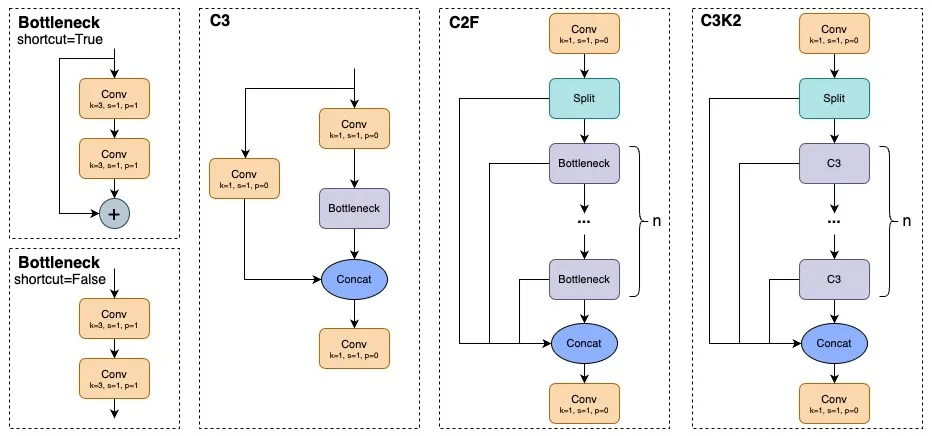
\includegraphics[scale=0.35]{gambar/C3k2.jpg}
  \caption{Bottleneck, C3, C2F, and C3K2 Modules}
  \label{fig:c3k2}
\end{figure}

The input features are transformed in the feedforward layer into a higher-dimensional space, allowing complex non-linear relationships to be captured more stably.

\subsection{MediaPipe}
\label{subsec:MediaPipe}

\emph{MediaPipe} is an open-source framework developed by Google for building efficient media processing pipelines, including image and video processing. This framework provides various modules that can be utilized for applications such as face detection, hand tracking, and pose estimation.

The \emph{MediaPipe} framework uses the concept of a "graph," where each node in the graph functions as a "calculator" that performs specific tasks, such as object detection, pose tracking, or image segmentation. The configuration of these nodes can be customized through \emph{GraphConfig}, which defines the topology and functionality of the entire system.

\begin{figure}[H]
  \centering
  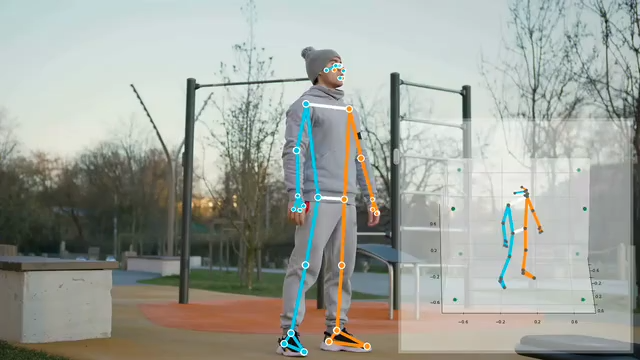
\includegraphics[scale=0.35]{gambar/MediaPipe3D.png}
  \caption{MediaPipe 3D}
  \label{fig:MediaPipe3D}
\end{figure}

One of the most well-known uses of \emph{MediaPipe} is human pose estimation using the \emph{MediaPipe Pose} module. This technique combines 2D pose estimation with a more complex humanoid model and uses optimization methods to calculate joint angles in 3D poses. This approach is effective in addressing depth ambiguity issues in 3D pose estimation and can work in real-time. The resulting 3D pose visualization shows each body joint as points and connecting lines between joints, providing a clear picture of the body's position and orientation in 3D space.

\vspace{5pt}
\subsubsection{MediaPipe Pose}
\label{subsubsec:MediaPipe Pose}

\emph{MediaPipe Pose} is a module within \emph{MediaPipe} specifically designed to detect and track human poses in real-time. Using advanced machine learning models, \emph{MediaPipe Pose} can identify up to 33 reference points on the human body, allowing the system to understand and respond to user movements quickly and accurately.

\begin{figure}[H]
  \centering
  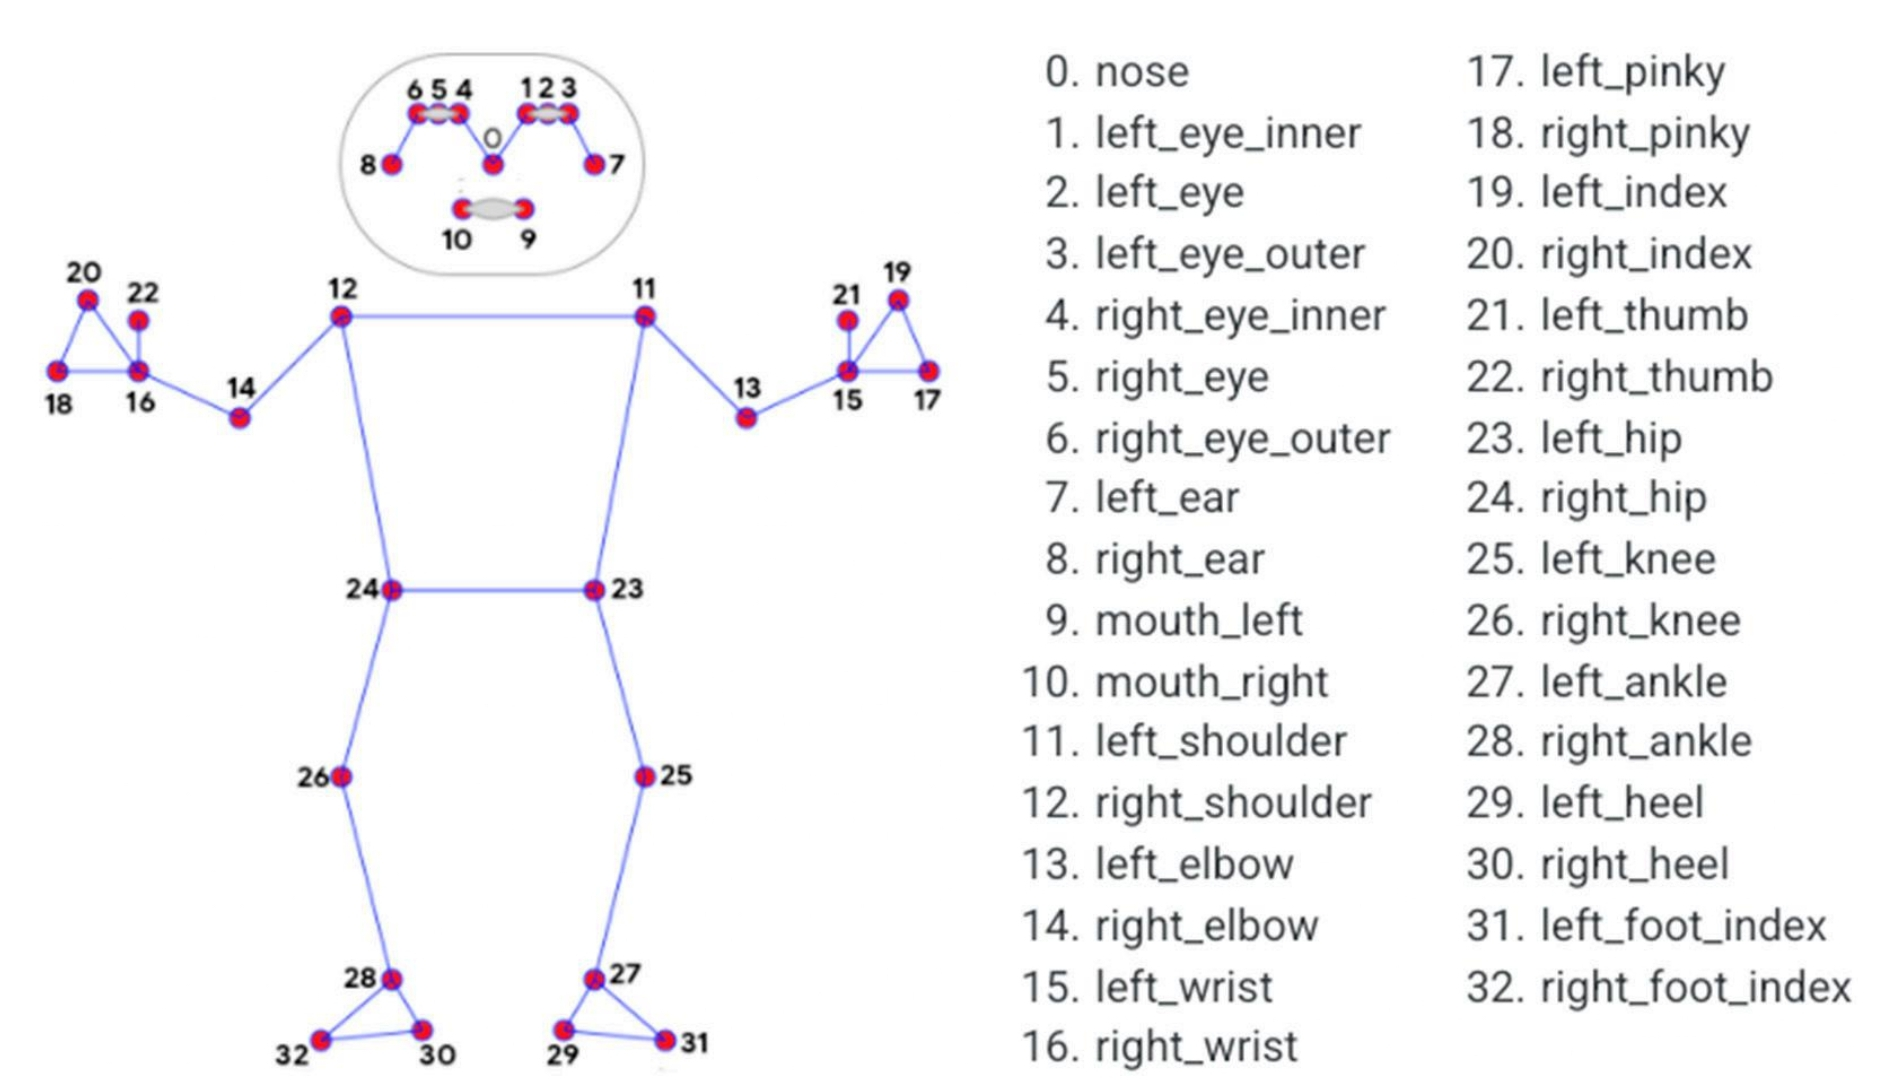
\includegraphics[scale=0.5]{gambar/mp_pose.jpg}
  \caption{MediaPipe Pose}
  \label{fig:mp_pose}
\end{figure}

\subsection{Classification Performance}
\label{subsec:Classification Performance}

\emph{Classification performance} refers to the ability of a model to classify input data into the correct categories. The classification process requires evaluation to assess the effectiveness of the developed model, usually using a test dataset. One commonly used evaluation approach in the context of classification is the \emph{confusion matrix}, which provides a visualization of the model's performance in categorizing data accurately.

\begin{figure}[H]
  \centering
  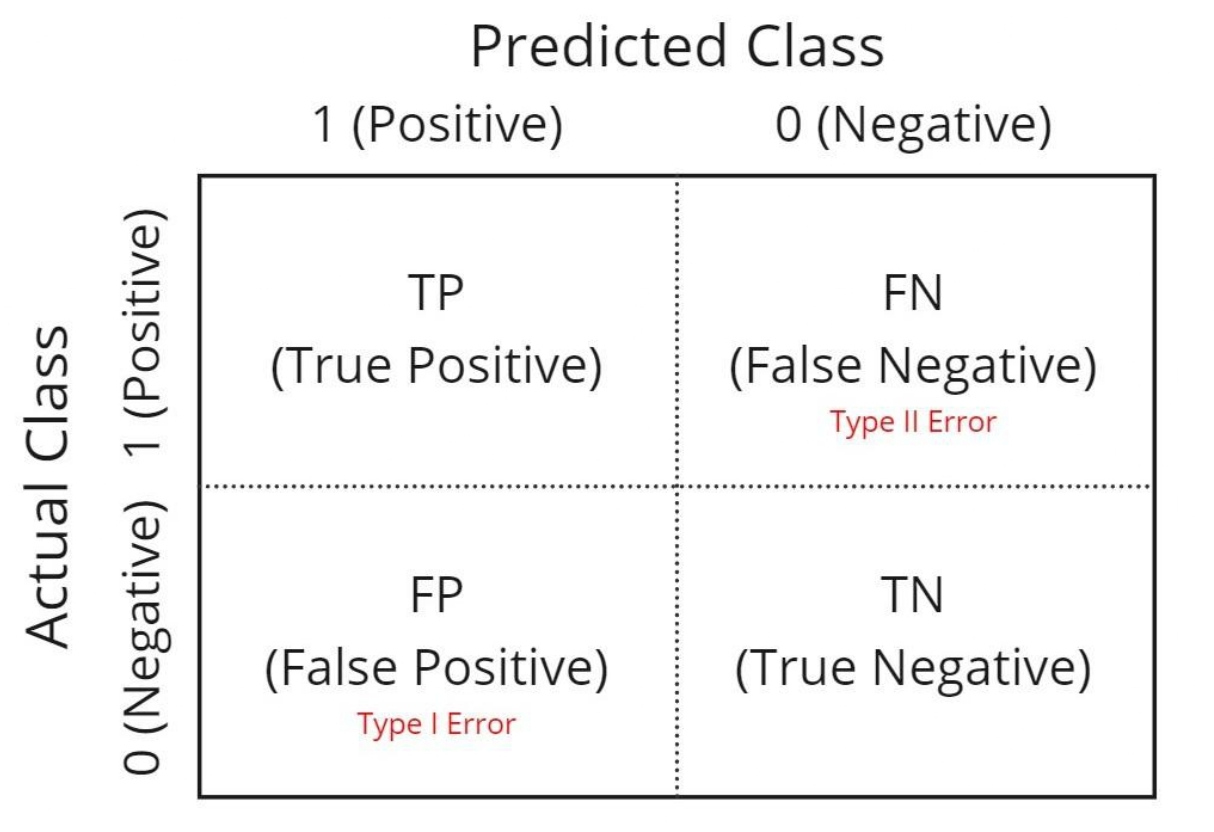
\includegraphics[scale=0.5]{gambar/Matrix Konfusi.jpg}
  \caption{Confusion Matrix.}
  \label{fig:confusion}
\end{figure}

The \emph{confusion matrix} is used to evaluate the performance of a binary classification model and displays four types of prediction results: \emph{True Positive} (TP), \emph{False Negative} (FN), \emph{False Positive} (FP), and \emph{True Negative} (TN). TP occurs when the model correctly predicts the positive class, while FN occurs when the model incorrectly predicts the negative class when it should be positive (also known as \emph{Type II Error}). FP occurs when the model incorrectly predicts the positive class when it should be negative (also known as \emph{Type I Error}), and TN occurs when the model correctly predicts the negative class.

\subsection{Evaluation Metrics}
\label{subsec:Evaluation Metrics}

Evaluation metrics serve as the basis for understanding and comparing the effectiveness of various algorithms and different scenarios. Through careful evaluation, accurate comparisons between different object detection techniques can be made, and the level of accuracy achieved can be properly assessed. This is crucial in selecting the most suitable algorithm for a specific detection task. Metrics such as \emph{accuracy}, \emph{precision}, and \emph{recall} are used to evaluate the effectiveness of a model in correctly detecting and identifying objects. Implementing these metrics is necessary to determine the most efficient model.

Additionally, accuracy analysis provides significant quantitative insights into the performance of object detection algorithms, as well as further details on the algorithm's ability to produce accurate detections. Errors identified through evaluation metrics are an important step in detection research, such as in the case of smoke detection. This identification facilitates understanding potential errors in the algorithm, which can then lead to improvements and enhancements in detection methods. Evaluation metrics are also utilized to support the optimization of algorithm hyperparameters.

In this research, various evaluation metrics such as \emph{precision}, \emph{recall}, and \emph{Mean Average Precision} (mAP) have been applied. By combining these evaluation methods, this research is designed to present a comprehensive analysis of the performance of the reviewed object detection algorithms. The explanation of the basic concepts of evaluation metrics is outlined as follows:

\vspace{5pt}
\subsubsection{Precision}
\label{subsubsec:precision}

\emph{Precision} is one of the main metrics used to measure how accurately the model's predictions match the detected objects. This metric indicates the proportion of true positive predictions (\emph{True Positive}) compared to the total positive predictions, both true (\emph{True Positive}) and false (\emph{False Positive}), expressed by the following equation:
\begin{equation}
  \mathrm{Precision} = \frac{TP}{TP + FP}
\end{equation}

Where \(TP\) (\emph{True Positive}): Correct prediction, i.e., detection of objects that match the ground truth, and \(FP\) (\emph{False Positive}): Incorrect prediction, i.e., detection of objects that do not match the ground truth.

\emph{Precision} is very useful in situations where false positive predictions need to be minimized. For example, in autonomous wheelchair applications, incorrect detection of humans can lead to dangerous actions, so \emph{precision} must be maintained at a high value.

\emph{Precision} is usually combined with other metrics, such as \emph{recall}, to provide a more complete picture of the model's performance.

\vspace{5pt}
\subsubsection{Recall}
\label{subsubsec:recall}

\emph{Recall} or sensitivity measures the model's ability to detect all objects present in an image or video. \emph{Recall} emphasizes how many objects that actually exist in the data (ground truth) are successfully detected by the model with the following equation:

\begin{equation}
  \mathrm{Recall} = \frac{TP}{TP + FN}
\end{equation}

Where \(TP\) (\emph{True Positive}): Correct prediction, i.e., objects that are correctly detected, and \(FN\) (\emph{False Negative}): Incorrect prediction, i.e., objects that exist but are not detected.

This metric is important when errors in failing to detect objects (\emph{false negative}) need to be minimized. In the context of developing an autonomous wheelchair, \emph{recall} is crucial because objects such as humans must always be detected to ensure the wheelchair can follow accurately.

\textbf{\emph{Precision and Recall Trade-off:}} In many cases, \emph{precision} and \emph{recall} have an inverse relationship. If the model is too conservative in making predictions, \emph{precision} will be high, but \emph{recall} will be low. Conversely, if the model is too lenient in detecting objects, \emph{recall} will be high, but \emph{precision} will decrease. Therefore, a balance between \emph{precision} and \emph{recall} is needed, which is usually expressed through other metrics such as \emph{F1-score}.

\vspace{5pt}
\subsubsection{Mean Average Precision (mAP)}
\label{subsubsec:mAP}

\emph{Mean Average Precision} (mAP) is a comprehensive metric used to measure the overall performance of an object detection model. \emph{mAP} is the average of the \emph{average precision} (AP) across all classes in the dataset.

\begin{equation}
  \mathrm{AP} = \int_0^1 P(r) \, dr
\end{equation}

Where \(P(r)\) is the \emph{Precision} as a function of \emph{recall} and \(dr\) is the differential of \emph{recall}.

AP is calculated by finding the area under the \emph{precision-recall} (PR) curve for each class. After calculating the AP for all classes, the average of these values gives the \emph{mAP}.

\begin{equation}
  \mathrm{mAP} = \frac{1}{N} \sum_{i=1}^{N} \mathrm{AP}_i
\end{equation}

Where \(N\) is the number of classes in the dataset and \(AP_i\) is the \emph{average precision} for the i-th class.

\emph{mAP} provides a broader view of the object detector's performance, as this metric considers both \emph{precision} and \emph{recall} simultaneously. The \emph{mAP} value will serve as a reference for evaluating the system's performance, such as detecting various objects like humans, obstacles, and the surrounding environment.

\vspace{5pt}
\subsubsection{Intersection over Union (IoU)}
\label{subsubsec:IoU}

\emph{Intersection over Union} (\emph{IoU}) is a metric used to evaluate the accuracy of object position detection performed by the model in image processing. The intersection area between the detection box generated by the model and the reference box, known as the \emph{Ground Truth}, is calculated to assess the model's performance. This ratio is obtained by comparing the area of overlap between the two boxes to the total area of their union. If the two boxes are treated as a single entity, \emph{IoU} provides a score indicating how accurately the model predicts the actual location of the object. The \emph{IoU} value increases as the proportion of the intersection area relative to the total union area increases.

\begin{figure}[H]
  \centering
  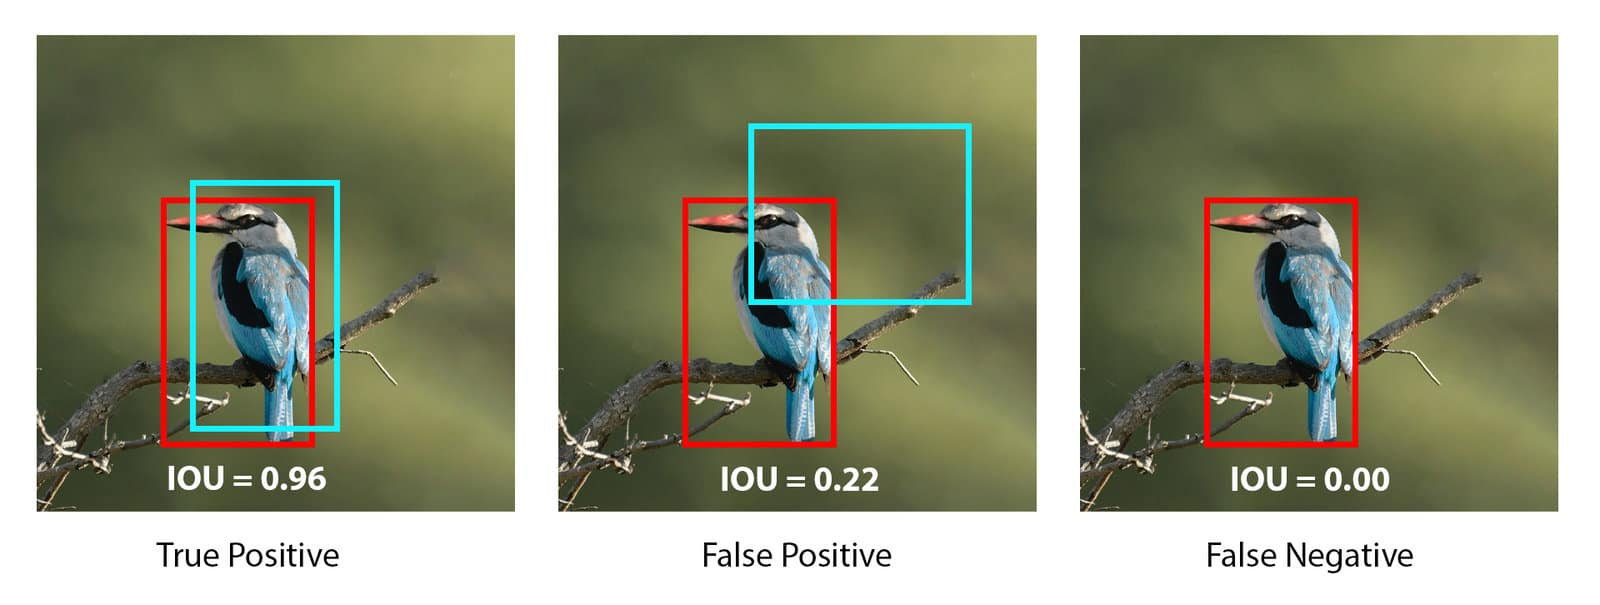
\includegraphics[scale=0.15]{gambar/IoU bbox.jpg}
  \caption{Intersection over Union.}
  \label{fig:IoU_bbox}
\end{figure}

The performance of the object detection model is evaluated by comparing the overlapping area between the predicted bounding box and the ground truth bounding box. The \emph{IoU} value ranges from 0 to 1, where a value closer to 1 indicates a higher level of accuracy in detecting and locating objects.

During the evaluation process, the bounding box generated by the model is compared to the ground truth bounding box, which is manually determined as the actual location of the object in the image. The \emph{IoU} is calculated by dividing the area of overlap between the two bounding boxes by the total area of their union. The following equation is used to calculate the \emph{IoU} value:

\begin{equation}
  IoU = \frac{\left |A \bigcap B \right |}{\left | A \bigcup B \right |}
\end{equation}

\emph{IoU} is chosen as a measurement tool because of its ability to provide a clear assessment of how accurately the model identifies and bounds objects under various conditions, including variations in size, orientation, and context of objects in the image. A higher \emph{IoU} value indicates that the model can reliably detect and identify objects with a high level of precision.

\subsection{BoT-SORT}

BoT-SORT is a multi-object tracking (MOT) method developed with a tracking-by-detection approach. Essentially, this method leverages several techniques from previous algorithms, particularly ByteTrack, to provide more advanced tracking. Improvements in this method aim to enhance tracking performance in both dynamic and static environments by refining several key components, which will be detailed as follows \cite{aharon2022botsortrobustassociationsmultipedestrian}:

\vspace{5pt}
\subsubsection{Kalman Filter}
\label{subsubsec:Kalman Filter}

The Kalman Filter (KF) is used to predict the location of objects in the next frame based on previous movements. BoT-SORT utilizes a KF with a state vector that includes the object's center coordinates ($x_c$, $y_c$), width ($w$), height ($h$), and the rate of change (velocity) of these variables ($\dot{x_c}$, $\dot{y_c}$, $\dot{w}$, $\dot{h}$) \cite{bewley2016simple, wojke2017simple}. This state vector is defined as:

\begin{equation}
  \begin{split}
    \vb*{x}_k = [x_{c}{\scriptstyle(k)}, y_{c}{\scriptstyle(k)}, w{\scriptstyle(k)}, h{\scriptstyle(k)}, \\        
    \dot{x_{c}}{\scriptstyle(k)}, \dot{y_{c}}{\scriptstyle(k)}, \dot{w}{\scriptstyle(k)}, \dot{h}{\scriptstyle(k)}]^\top
  \end{split}
\end{equation}

\begin{equation}
  \vb*{z}_k = [z_{x_c}{\scriptstyle(k)}, z_{y_c}{\scriptstyle(k)}, z_{w}{\scriptstyle(k)}, z_{h}{\scriptstyle(k)}]^\top
\end{equation}

The process noise matrix ($\mathbf{Q}_k$) and measurement noise matrix ($\mathbf{R}_k$) are adjusted to be more sensitive to changes within frames, which helps improve tracking accuracy. The matrices $\mathbf{Q}_k$ and $\mathbf{R}_k$ are defined as follows:

\begin{equation}
  \begin{split}
    \vb*{Q}_k = diag\big{(} (\sigma_{p} \hat{w}_{k-1|k-1})^2, (\sigma_{p} \hat{h}_{k-1|k-1})^2, \\
    (\sigma_{p} \hat{w}_{k-1|k-1})^2, (\sigma_{p} \hat{h}_{k-1|k-1})^2, \\
    (\sigma_{v} \hat{w}_{k-1|k-1})^2, (\sigma_{v} \hat{h}_{k-1|k-1})^2, \\ 
    (\sigma_{v} \hat{w}_{k-1|k-1})^2 ,(\sigma_{v} \hat{h}_{k-1|k-1})^2\big{)}
  \end{split}
\end{equation}

\begin{equation}
  \begin{split}
      \vb*{R}_k = diag\big{(}(\sigma_{m} \hat{w}_{k|k-1})^2, (\sigma_{m} \hat{h}_{k|k-1})^2, \\
      (\sigma_{m} \hat{w}_{k|k-1})^2, (\sigma_{m} \hat{h}_{k|k-1})^2\big{)} 
  \end{split}
\end{equation}

With these changes, the bounding box predictions are more accurate compared to traditional Kalman Filter methods, as evidenced by the increased HOTA (Higher Order Tracking Accuracy) values.

\begin{figure}[H]
  \centering
  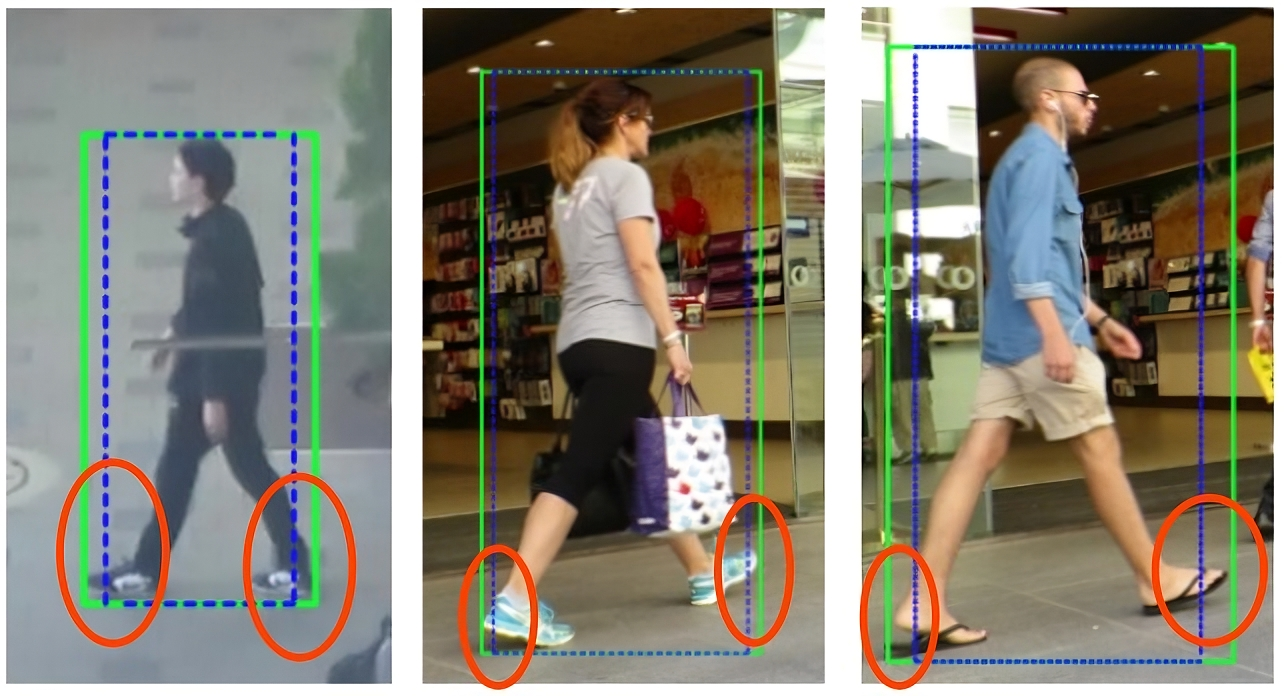
\includegraphics[scale=0.19]{gambar/KF_width.png}
  \caption{Kalman Filter bbox.}
  \label{fig:KF width}
\end{figure}

Visualization of the bounding box shape compared to the widely used Kalman filter~\cite{wojke2017simple} (dashed blue) and the proposed Kalman filter (green). It is evident that the width of the bounding box generated by the proposed Kalman filter is more appropriate for the object. The dashed blue bounding box cuts off part of the object's legs (in red), while the green bounding box reaches the desired width.

\vspace{5pt}
\subsubsection{\emph{Camera Motion Compensation} (CMC)}
\label{subsubsec:Camera Motion Compensation}

Trackers based on tracking-by-detection often face issues of ID switches or false negatives due to camera motion, especially in dynamic situations. BoT-SORT implements Camera Motion Compensation (CMC) techniques by utilizing affine transformation to compute the transformation between two frames. By extracting image keypoints \cite{shi1994good}, and then using sparse optical flow ~\cite{Bouguet1999PyramidalIO} for feature tracking with local outlier rejection based on translation. The affine matrix $\vb*{A}_{k-1}^k\in \mathbb{R}^{2 \times 3}$ is solved using the RANSAC method ~\cite{fischler1981random}. The use of sparse registration techniques allows for the exclusion of dynamic objects in the scene based on detection, thus having the potential to estimate background motion more accurately.

\begin{equation}
  \begin{aligned}
      & \vb*{A}_{k-1}^k = 
      \begin{bmatrix}
          \vb*{M}_{2x2} | \vb*{T}_{2x1}
      \end{bmatrix} = 
      \begin{bmatrix}
          a_{11}\;a_{12}\;a_{13} \\ a_{21}\;a_{22}\;a_{23} \\ 
      \end{bmatrix}
  \end{aligned}
\end{equation}
\begin{equation}
  \begin{aligned}
  {
      \vb*{\tilde{M}}}^k_{k-1} = 
      \begin{bmatrix}
      \vb*{M} & \vb*{0} & \vb*{0} & \vb*{0} \\
      \vb*{0} & \vb*{M} & \vb*{0} & \vb*{0} \\
      \vb*{0} & \vb*{0} & \vb*{M} & \vb*{0} \\
      \vb*{0} & \vb*{0} & \vb*{0} & \vb*{M}
      \end{bmatrix}, \; 
      \tilde{\vb*{T}}_{k-1}^k = 
      \begin{bmatrix}a_{13}\\a_{23}\\ 0\\ 0\\ \vdots \\ 0\end{bmatrix}
  \end{aligned}
\end{equation}
\begin{equation}
  \begin{aligned}
      \hat{\vb*{x}}^\prime_{k|k-1} = \tilde{\vb*{M}}_{k-1}^k \hat{\vb*{x}}_{k|k-1} + \tilde{\vb*{T}}_{k-1}^k \\
  \end{aligned}
\end{equation}
\begin{equation}
    {{\vb*{P}}}^{\prime}_{k|k-1} = 
    \tilde{\vb*{M}}_{k-1}^k {\vb*{P}}_{k|k-1} {\tilde{\vb*{M}}_{k-1}}^{k^\top}
    \label{eq:cmc_cov}        
\end{equation}

Where $\vb*{M}\in \mathbb{R}^{2 \times 2}$ is a matrix containing the scale and rotation components of the affine matrix $\vb*{A}$, and $T$ contains the translation components. A mathematical trick is used by defining $\tilde{\vb*{M}}^k_{k-1}\in \mathbb{R}^{8 \times 8}$ and $\tilde{\vb*{T}}_{k-1}^k\in \mathbb{R}^{8}$. Subsequently, $\hat{\vb*{x}}_{k|k-1}$ and $\hat{\vb*{x}}^\prime_{k|k-1}$ are defined as the state prediction vectors of the Kalman Filter (KF) at time $k$, before and after camera motion compensation, respectively, while $\vb*{P}_{k|k-1}$ and $\vb*{P'}_{k|k-1}$ are defined as the KF covariance matrices before and after correction. After that, $\hat{\vb*{x}}^\prime_{k|k-1}$ and ${{\hat{\vb*{P}}}^{\prime}}_{k|k-1}$ are used in the Kalman Filter update step as follows.

\begin{equation}
  \begin{aligned}
  & \vb*{K_k} =  {{\vb*{P}}}^{\prime}_{k|k-1} \vb*{H}_k^\top (\vb*{H}_k  {{\vb*{P}}}^{\prime}_{k|k-1} \vb*{H}_k^\top + \vb*{R}_k)^{-1} \\
  & \hat{\vb*{x}}_{k|k} = \hat{\vb*{x}}^\prime_{k|k-1} + \vb*{K}_k (\vb*{z}_k - \vb*{H}_k \hat{\vb*{x}}^\prime_{k|k-1}) \\
  & \vb*{P}_{k|k} = (\vb*{I}- \vb*{K}_k \vb*{H}_k)  {{\vb*{P}}}^{\prime}_{k|k-1}
  \end{aligned}
  \label{eq:cmc_update_kf}
\end{equation} 

In high-speed scenarios, full correction of the state vector, including velocity components, is crucial. If the camera moves slowly compared to the frame rate, the correction in equation \ref{eq:cmc_cov} can be ignored. After compensating for rigid camera motion and assuming the object's position changes only slightly from one frame to the next, in high frame rate applications, when detections are missed, trajectory prediction can be performed using the KF prediction step, allowing for a more continuous trajectory display and higher MOTA.

Visualization of bounding box (BB) predictions from tracklets is used for association with new detection BBs based on maximum IoU criteria. (a.1) and (b.1) show predictions from the Kalman Filter (KF). (a.2) and (b.2) show predictions from the KF after camera motion compensation. In image (b.1), a scenario is shown where ignoring camera motion can lead to IDSWs or FNs. Conversely, in image (b.2), the prediction aligns with the desired location, and the association is successfully made. Figure \ref{fig:cmc} is generated from the MOT17 sequence \cite{milan2016mot16}, which includes camera movement due to a vehicle maneuvering to the right.

\begin{figure}[H]
  \centering
  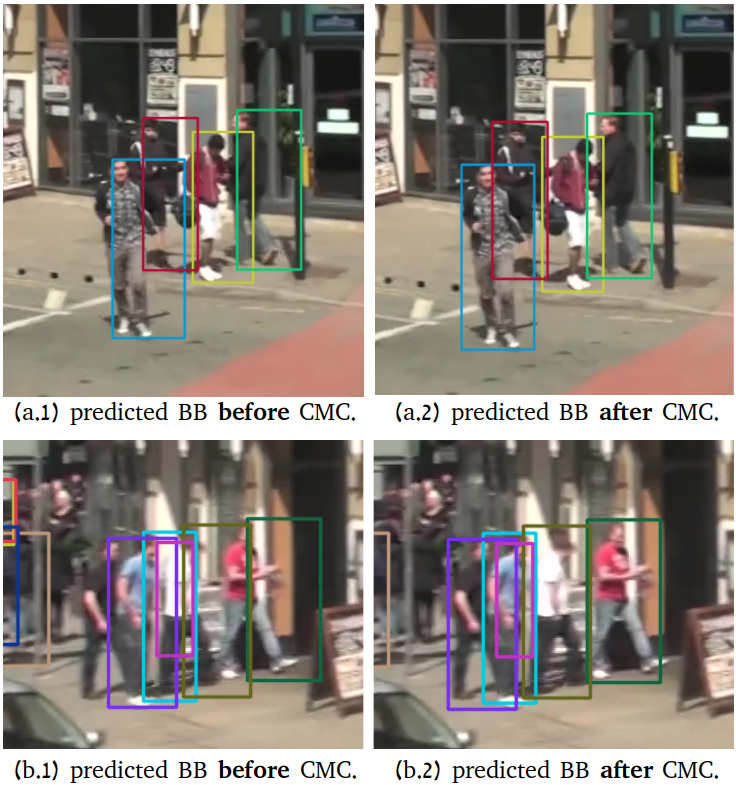
\includegraphics[scale=0.33]{gambar/cmc_pred.png}
  \caption{Camera Motion Compensation}
  \label{fig:cmc}
\end{figure}

\vspace{5pt}
\subsubsection{IoU - Re-ID Fusion}
\label{subsubsec:IoU - Re-ID Fusion}

Re-ID features are integrated to leverage advancements in visual object representation. Re-ID features are extracted using FastReID with the ResNeSt50 backbone \cite{he2020fastreid, zhang2020resnest}, and an exponential moving average (EMA) mechanism is used to update the tracklet appearance status \cite{wang2020towards}. The appearance status update is performed using the following formula:

\begin{equation}
e_i^k = \alpha e_i^{k-1} + (1 - \alpha) f_i^k
\end{equation}

Where $e_i^k$ is the appearance status for the $i$-th tracklet at frame $k$, $f_i^k$ is the current detection appearance embedding, and $\alpha=0.9$ is the momentum term.

The fusion of motion (IoU) and appearance (cosine similarity) information is performed as follows. First, candidates with low cosine similarity or those too far based on IoU scores are rejected. Next, the minimum value in each matrix element is used as the final value of the cost matrix $C$. The IoU-ReID fusion pipeline can be formulated as follows:

\begin{equation}
  \begin{aligned}
  & \hat{d}_{i, j}^{cos} = 
    \begin{cases}
      0.5 \cdot d_{i, j}^{cos}, \text{($d_{i, j}^{cos} < \theta_{emb})$ $\land$ $(d_{i, j}^{iou} < \theta_{iou})$}\\
      1, \text{otherwise}
    \end{cases} \\
  \end{aligned}
  \label{eq:min_dist}        
\end{equation}

\begin{equation}
  C_{i, j} = \min\{d_{i, j}^{iou}, \hat{d}_{i, j}^{cos}\}
\end{equation}

\begin{equation}
  \begin{aligned}
  \hat{b} = 
    \begin{cases}
      0, \quad\quad \Delta data \neq 0 \\
      1, \quad \neg ( \hat{t} \in [0, t] \lor b ) \\
      b, \quad\quad \text{otherwise}\\
    \end{cases}
  \end{aligned}
\end{equation}
  
Where $C_{i, j}$ is the element $(i, j)$ of the cost matrix $C$. $d_{i, j}^{iou}$ is the IoU distance between the $i$-th tracklet bounding box prediction and the $j$-th detection bounding box, representing the motion cost. $d_{i, j}^{cos}$ is the cosine distance between the average appearance descriptor of the $i$-th tracklet and the new detection descriptor of the $j$-th detection. $\hat{d}_{i, j}^{cos}$ is the new appearance cost used. $\theta_{iou}$ is the proximity threshold, set at 0.5, to reject unlikely tracklet and detection pairs. $\theta_{emb}$ is the appearance threshold, used to separate positive associations from the tracklet appearance state and detection embedding vector from negative associations.
The linear assignment problem of high-confidence detections, i.e., the first association step, is solved using the Hungarian algorithm~\cite{kuhn1955hungarian} and based on the cost matrix $C$, formed using Equation~\ref{eq:min_dist}.

\subsection{RoboFlow}
\label{subsec:RoboFlow}

\emph{RoboFlow} is a platform that supports efficient and effective data processing. Through various features provided, from data annotation to model evaluation, \emph{RoboFlow} ensures that every stage in the machine learning workflow can be carried out more structured and easily integrated with existing frameworks. Model performance improvements can be developed without being burdened by technical complexities in data preparation.

\emph{RoboFlow} facilitates the image annotation process through intuitive tools, accelerating the creation of labels for datasets. Images in the dataset are automatically modified through data augmentation to create variations that enhance the robustness of the trained model. Support for conversion between various popular dataset formats is also provided, simplifying data preparation for various machine learning algorithms. Additionally, functions for splitting the dataset into training, validation, and testing sets for model validation are available.

\emph{RoboFlow} also offers integration with many popular machine learning frameworks such as \emph{TensorFlow}, \emph{PyTorch}, and \emph{YOLO}, which includes:

\begin{itemize}
    \item \emph{Data Export}: Datasets can be easily exported in formats ready to be used by machine learning frameworks.
    \item \emph{Model Training}: The platform allows direct model training using the prepared and optimized dataset.
    \item \emph{Model Evaluation}: Model performance is measured using metrics that help in understanding and adjusting the model's effectiveness as needed.
\end{itemize}

\subsection{OBS Studio}
\label{subsec:OBS Studio}

\emph{OBS Studio} is an open-source software designed for video streaming and recording. In this project, \emph{OBS Studio} is used to document and analyze the performance of the autonomous wheelchair during the testing phase. This software allows the selection of various video input sources, including webcams, which are used to visually record the entire testing process. With \emph{OBS Studio}, the testing process from start to finish can be fully recorded, allowing for the collection of rich and detailed visual data.

\subsection{ESP32 Devkit V1}
\label{subsec:ESP32 Devkit V1}

\emph{ESP32 Devkit V1} is a microcontroller equipped with wireless communication capabilities, including \emph{Wi-Fi} and \emph{Bluetooth}. In this project, \emph{ESP32 Devkit V1} is used as the main communication module for the autonomous wheelchair. This device allows the wheelchair to interact with external devices such as smartphones or computers through wireless networks.

One of the main advantages of this \emph{Devkit} is the numerous pins it has, allowing the microcontroller to be programmed for various tasks. These pins provide high flexibility in connecting various sensors and actuators needed. By utilizing these pins, the system can perform multiple tasks simultaneously, such as collecting data from sensors, controlling motors, and managing wireless communication.

\begin{figure}[H]
  \centering
  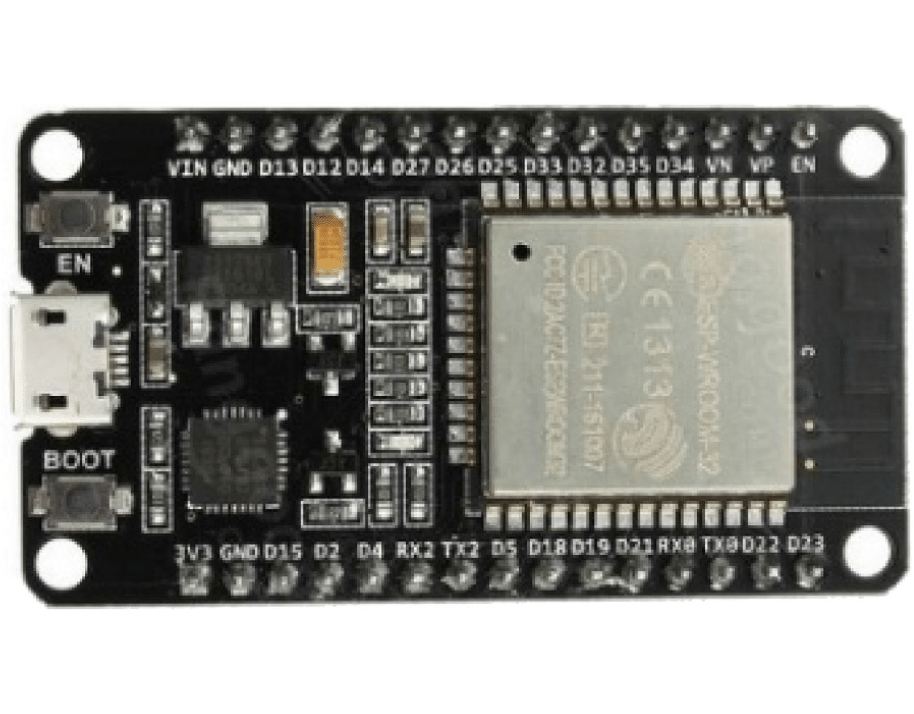
\includegraphics[scale=0.25]{gambar/ESP32-DEVKIT-V1-board.png}
  \caption{ESP32 Devkit V1}
  \label{fig:ESP32DevkitV1}
\end{figure}

This \emph{Devkit} is compatible with the \emph{Arduino IDE} using the \emph{C++} programming language, which is a commonly used platform. \emph{Arduino IDE} provides various libraries and support that facilitate the programming of \emph{ESP32} to control various connected hardware. With programming in \emph{C++}, efficient and structured code can be produced to perform various complex tasks, such as sensor data processing and motor control.

\subsection{Motor Driver H-Bridge}
\label{subsec:Motor}

\emph{Motor Driver H-Bridge} is a crucial electronic component in controlling the DC motor of the wheelchair. This component allows the adjustment of the motor's direction and speed, which is essential for wheelchair navigation under various conditions. By utilizing the \emph{H-Bridge}, the wheelchair motor can move forward, backward, or turn as needed.

\begin{figure}[H]
  \centering
  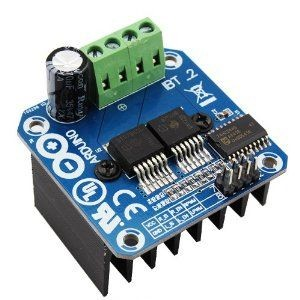
\includegraphics[scale=0.4]{gambar/Motor Driver H - bridge Bts.jpg}
  \caption{Motor Driver H-Bridge}
  \label{fig:MotorDriverH-Bridge}
\end{figure}

The use of \emph{H-Bridge} in the autonomous system allows real-time adjustment of the wheelchair's movement based on information received from sensors. This enables the wheelchair to follow the user's movements with high precision. The ability to navigate independently is crucial in ensuring that the wheelchair can operate safely and efficiently in various environments.

\subsection{KY-123 Electric Wheelchair}
\label{subsec:KY-123}

The \emph{KY-123} electric wheelchair is used as the main platform in the development of the autonomous wheelchair in this research. This wheelchair is equipped with integrated motors and controllers, allowing further modifications to support the designed autonomous system.

With the addition of sensors, cameras, and other hardware, the \emph{KY-123} wheelchair is expected to perform autonomous functions, including the ability to follow the user's movements independently. The integration between hardware and software on the \emph{KY-123} is a key element in achieving a reliable and effective system. These modifications aim to enhance mobility and ease of use for individuals with physical limitations, ensuring optimal performance in various usage scenarios.

\begin{figure}[H]
  \centering
  \includegraphics[scale=0.05]{gambar/kursi roda.png}
  \caption{KY-123 Electric Wheelchair}
  \label{fig:KYElectricWheelchair}
\end{figure}